\documentclass{article}

\usepackage[utf8]{inputenc}
\usepackage{graphicx}
\usepackage[margin=3cm]{geometry}

\title{MontePyton}
\author{Aleksander Trzciński, Dominik Mrozek, Oliwier Maj, Emilia Myrta, Natalia Kwiecień}
\date{October 2022}

\begin{document}
\maketitle

\section{Emilia Myrta}

Math expression:

\[x^2 - y^2 = (x + y)(x - y)\]

Photo~\ref{fig:dog}.

\begin{figure}[htbp]
    \centering
    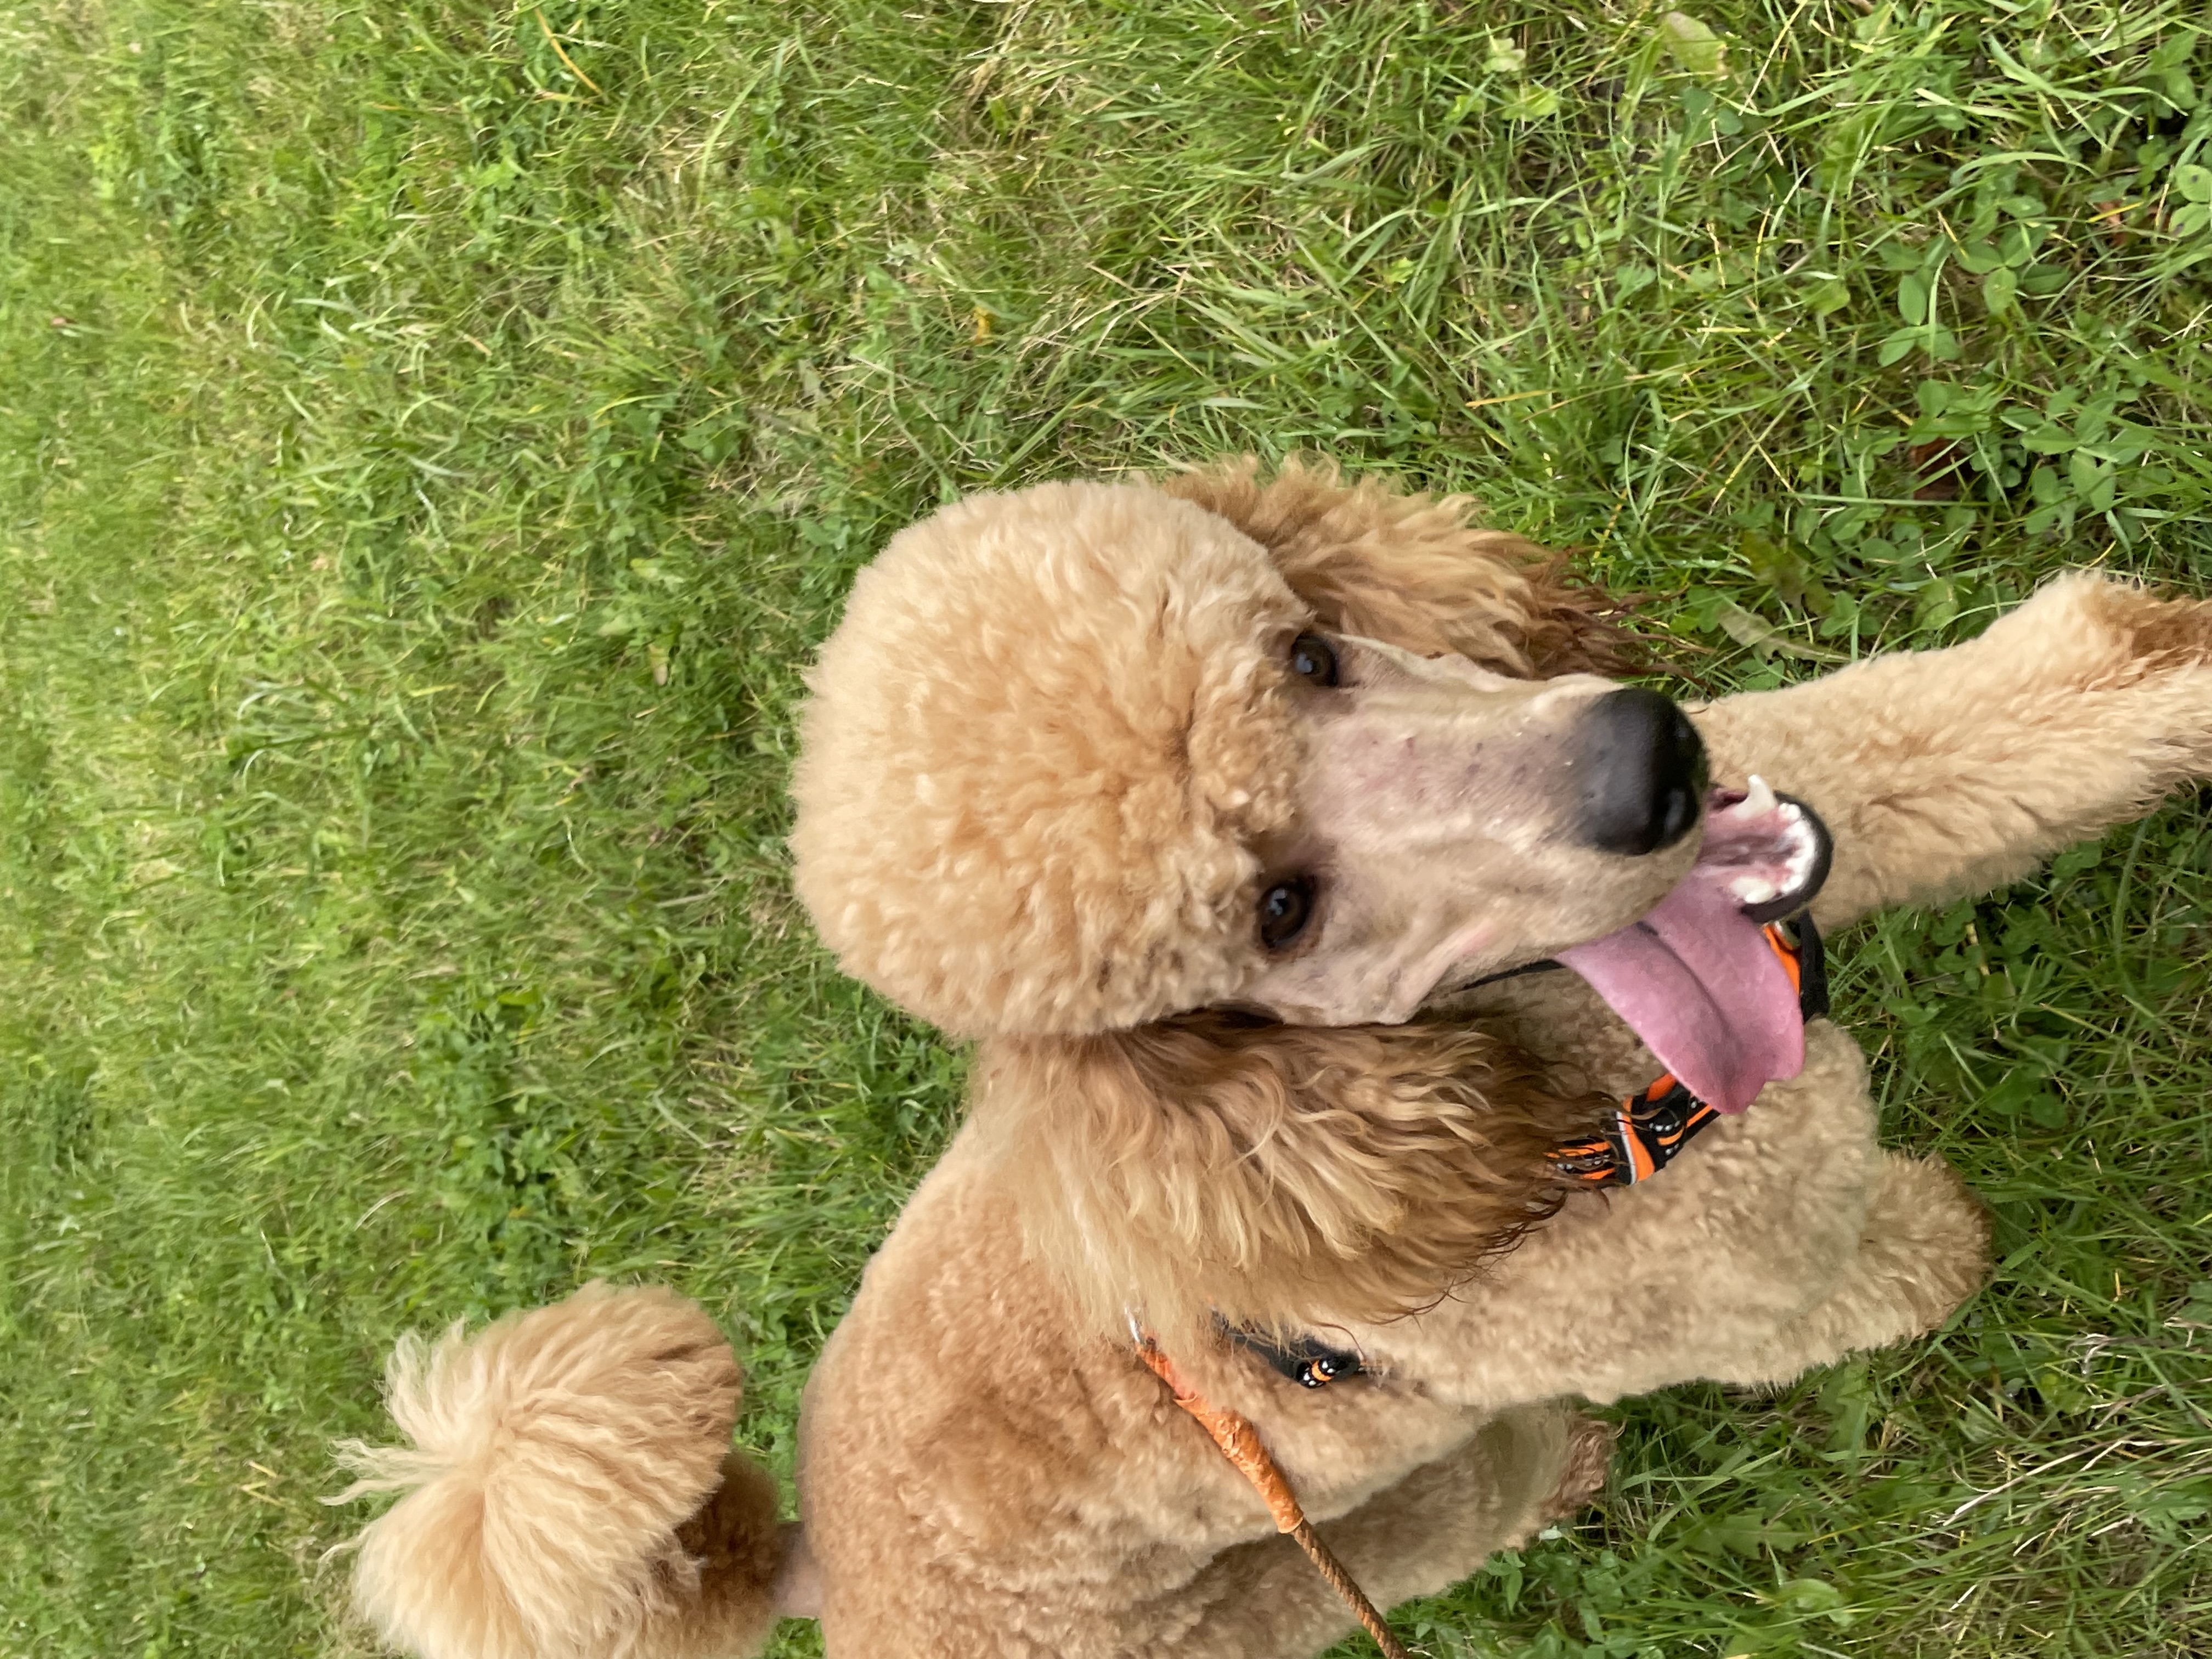
\includegraphics[width=0.4\textwidth]{Pictures/zdjecie_emilia.jpg}
    \caption{Dog.}
    \label{fig:dog}
\end{figure}

Table~\ref{tab:test}.

\begin{table}[htbp]
\centering
\begin{tabular}{|l|l|l|l|l|l|}
\hline
Column 1 & Column 2 & Column 3 & Column 4 & Column 5 & Column 6 \\ \hline
Row 2    & 0        & 1        & 2        & 3        & 4        \\ \hline
Row 3    & 1        & 2        & 3        & 4        & 5        \\ \hline
\end{tabular}
\label{tab:test}
\caption{}
\end{table}

List of largest cities by population (2018):
\begin{enumerate}
  \item Tokyo, Japan - 37,468,000 
  \item Delhi, India - 28,514,000 
  \item Shanghai, China	- 25,582,000 	
\end{enumerate}

\begin{itemize}
  \item Number 1
  \item Number 2
  \item Number 3
\end{itemize}

\begin{flushleft}
Boosting and encouraging use of \underline{energy efficiency technologies} would lead to reduced energy needs for powering, heating, and cooling of homes, businesses, and industries. This would be effective in \textbf{reducing global warming} as the problem is largely contributed to by the energy used for cooling, heating, and power services in industries, businesses, and homes. In the transportation sector for instance, \underline{switching to fuels that are low in carbon}, and improving fuel efficiency in terms of miles per gallon would reduce the amount of heat-trapping emissions released into the atmosphere.\par
Additionally, \textbf{\textit{revving up renewable energy}} could reduce global warming. The vast majority of energy needs worldwide can be potentially met by such renewable sources of energy as bioenergy, geothermal, wind, and solar energy that apart from reducing pollution, would also \emph{create jobs}. According to the Environmental Protection Agency’s 2012 report, \textbf{coal-fired power plants produce approximately \emph{25 percent} of total U.S. global warming emissions} while natural gas-fired power plants produce 6 percent of total emissions. In contrast, most renewable energy sources produce little to no global warming emissions. Conclusively, boosting energy efficiency and adopting renewable energy would reduce global warming.
\end{flushleft}

\vspace{0.1cm}
\section{Oliwier Maj}

I love mushrooms and picking them. (Figure~\ref{fig:grzyb}).

\begin{figure}[htbp]
    \centering
    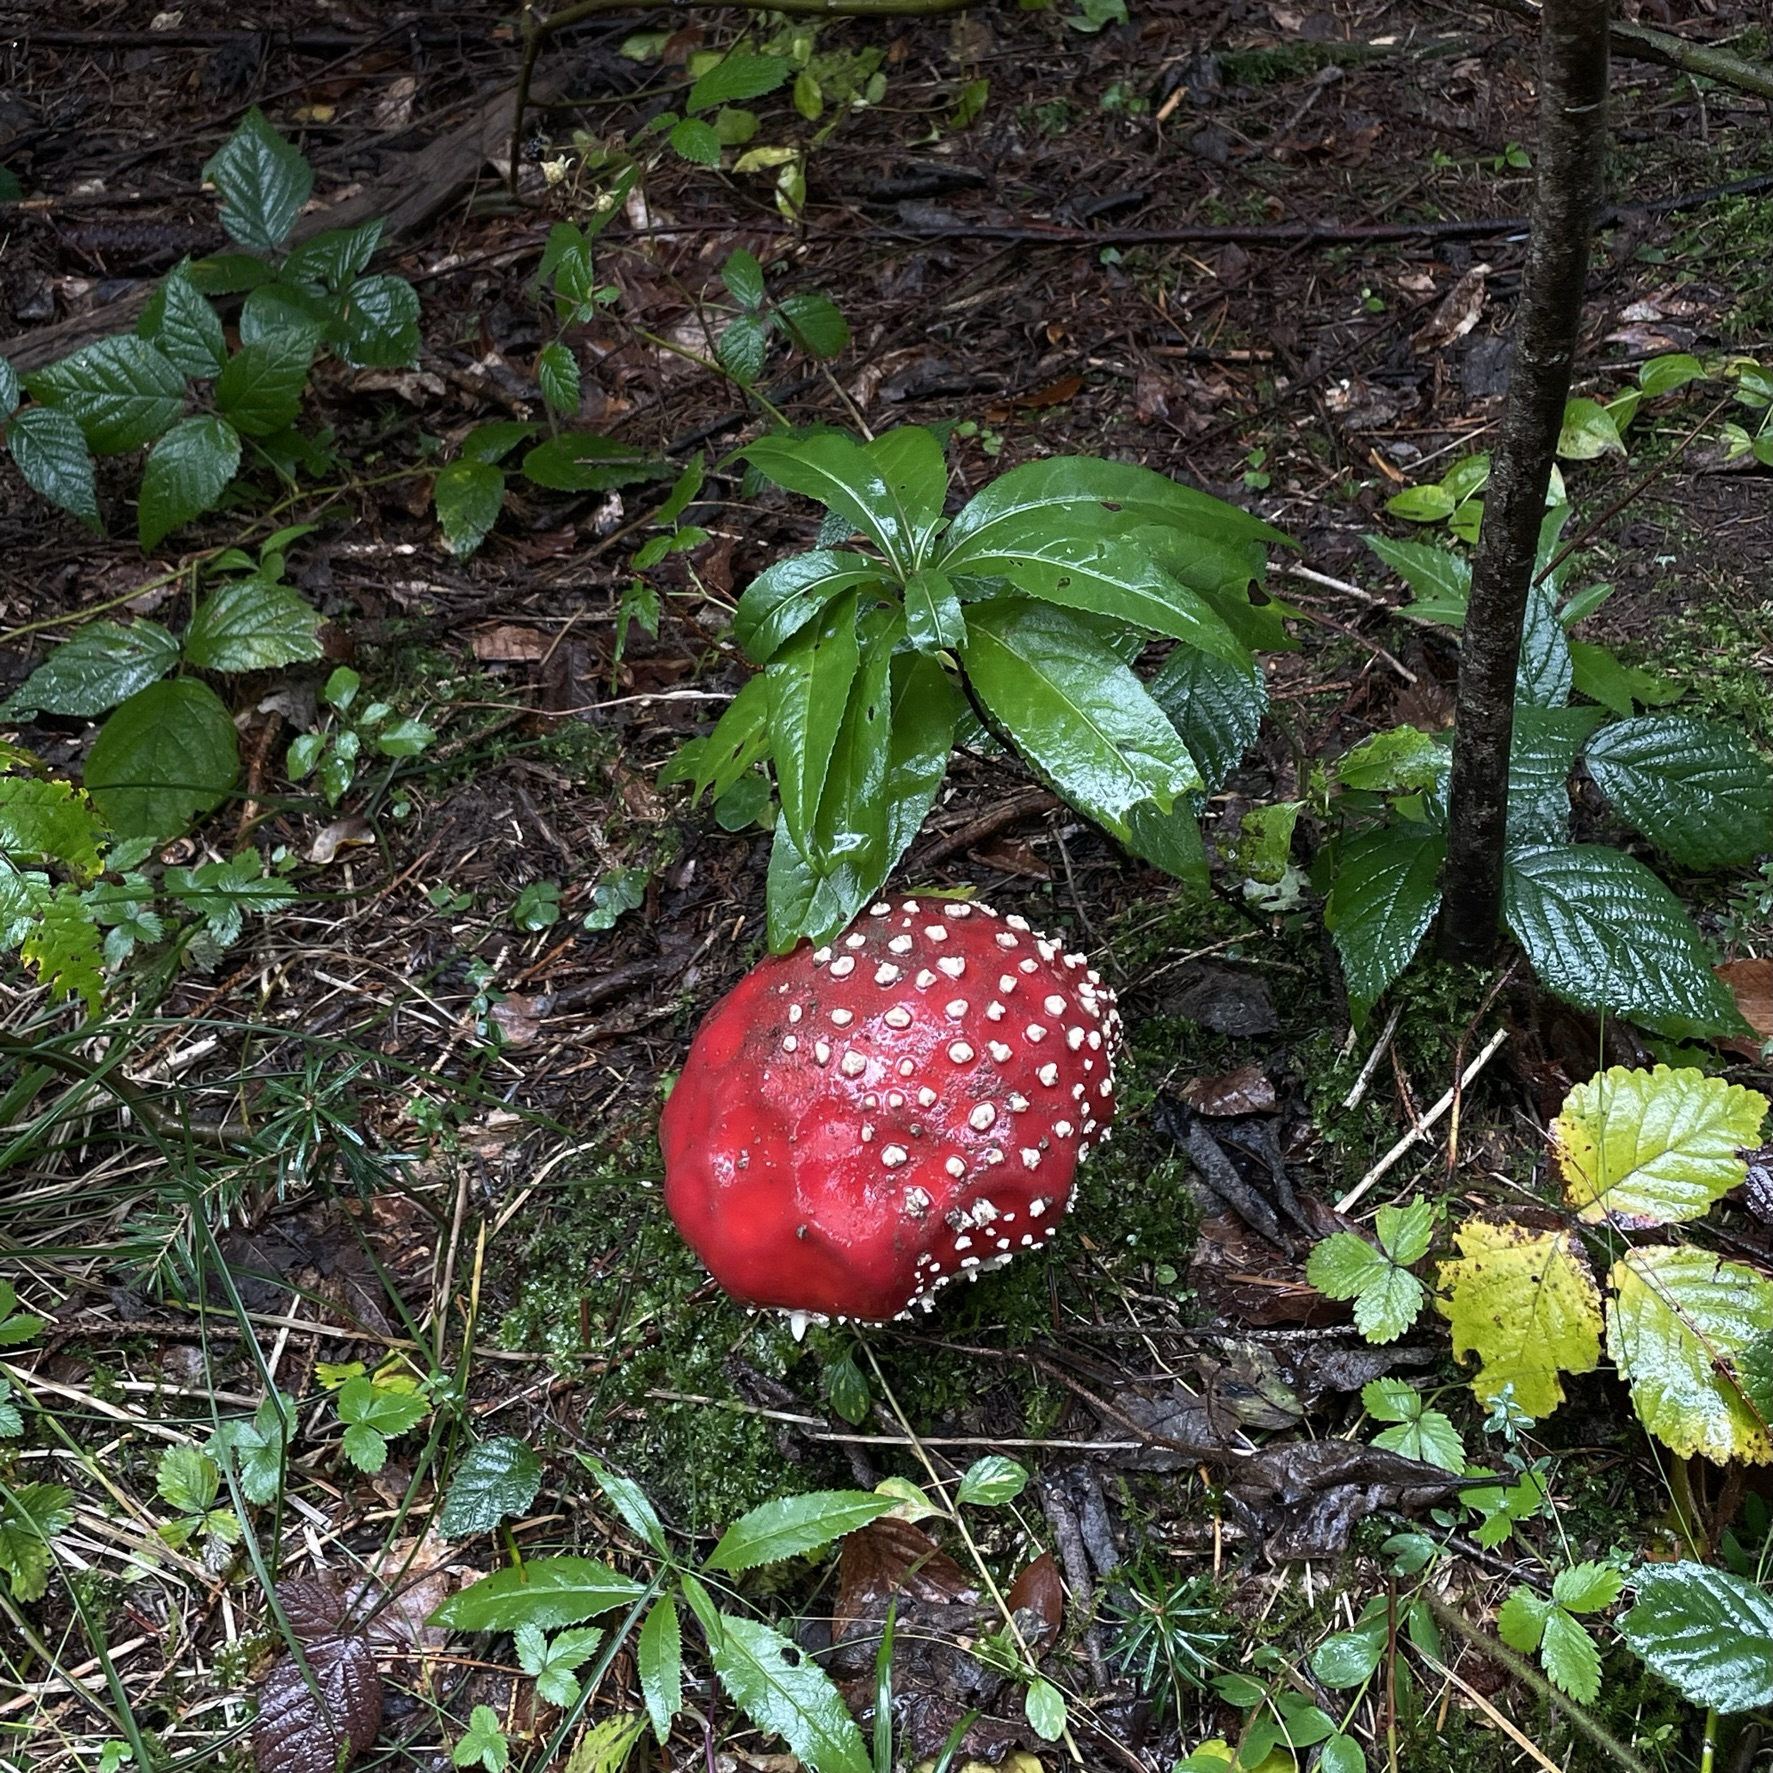
\includegraphics[width=0.6\textwidth]{Pictures/grzyb.jpeg}
    \caption{My toadstool.}
    \label{fig:grzyb}
\end{figure}

I would love to pass maths this year. Here is my favourite equation:\[(x+y)^2=x^2+y^2+2xy\]

\vspace{5.0cm}

Table~\ref{tab:tabulita} is tick-tack-toe game.\par
\begin{table}[htbp]
    \centering
    \begin{tabular}{||c|c|c||} \hline\hline
        O & X & O \\ \hline
        O & X & X \\ \hline
        X & O & X \\ \hline \hline
    
    \end{tabular}
    \label{tab:tabulita}
    \caption{Its a tie. :)}
\end{table}

\vspace{1.0cm}

The rank of tea flavors according to me.
\begin{enumerate}
    \item Jasmin
    \item Mango-mint
    \item Raspberry-passion fruit
\end{enumerate}
\vspace{0.5cm}

Fun words:
\begin{itemize}
    \item[*] blackout
    \begin{itemize}
        \item [-] help 
        \item [-] me
    \end{itemize}
    \item[*] toadstool
    \item[*] motherlode
\end{itemize}

\vspace{2.0mm}

\begin{flushleft}
\begingroup
\raggedleft
"Lorem ipsum dolor sit \textbf{amet, consectetur adipiscing elit}, sed do eiusmod tempor incididunt ut labore et dolore magna aliqua. Ut enim ad minim veniam,\par quis nostrud exercitation ullamco laboris nisi ut aliquip ex ea commodo consequat. Duis aute irure dolor in reprehenderit in \textbf{voluptate} velit esse cillum dolore eu fugiat nulla pariatur. Excepteur sint occaecat cupidatat non proident, sunt in culpa qui officia deserunt mollit anim id est laborum."

\endgroup

\vspace{0.5cm}

\begingroup
\raggedright
"Sed ut perspiciatis unde omnis iste natus error sit voluptatem accusantium doloremque laudantium,\textbf{\textit{totam rem aperiam}}, eaque ipsa quae ab illo inventore veritatis et quasi architecto beatae vitae dicta sunt explicabo. \underline{Nemo enim ipsam voluptatem quia voluptas sit aspernatur aut odit aut fugit}, sed quia consequuntur magni dolores eos qui ratione voluptatem sequi nesciunt.\par Neque porro quisquam est, qui dolorem ipsum quia dolor sit amet, consectetur, adipisci velit, sed quia non numquam eius modi tempora incidunt ut labore et dolore magnam aliquam quaerat voluptatem. Ut enim ad minima veniam, quis \textit{nostrum ullam \emph{textitcorporis} suscipit} laboriosam, nisi ut aliquid ex ea commodi consequatur? Quis autem vel eum iure reprehenderit qui in ea voluptate velit esse quam nihil molestiae consequatur, vel illum qui dolorem eum fugiat quo voluptas nulla pariatur?"

\endgroup
\end{flushleft}
\vspace{0.1cm}
\newpage
\section{Dominik Mrozek}

Fundamental trigonometric equation:
\[(sinx)^2+(cosx)^2=1\]

Photo~\ref{fig:panda}.
\begin{figure}[htbp]
    \centering
    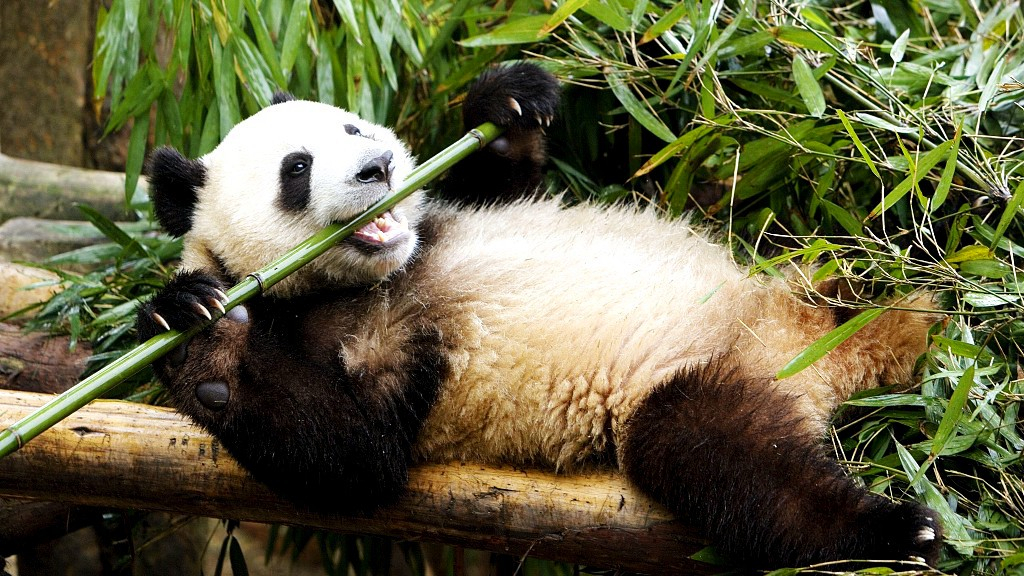
\includegraphics[width=1\textwidth]{Pictures/panda.jpg}
    \caption{Panda eating bamboo.}
    \label{fig:panda}
\end{figure}

Table~\ref{tab:tabelka}.
\begin{table}[htbp]
\centering
\begin{tabular}{|l|l|l|}
\hline
\textbf{\#} & \textit{\textbf{Country}} & \textit{\textbf{GDP per Capita (US \$)}} \\ \hline
\textbf{1}  & Monaco                    & 190,512                                  \\ \hline
\textbf{2}  & Liechtenstein             & 180,366                                  \\ \hline
\textbf{3}  & Luxembourg                & 115,873                                  \\ \hline
\textbf{4}  & Switzerland               & 87,097                                   \\ \hline
\textbf{5}  & Macao                     & 86,117                                   \\ \hline
\textbf{6}  & Ireland                   & 85,267                                   \\ \hline
\textbf{7}  & Norway                    & 67,389                                   \\ \hline
\textbf{8}  & United States             & 63,543                                   \\ \hline
\textbf{9}  & Denmark                   & 61,063                                   \\ \hline
\textbf{10} & Singapore                 & 59,797                                   \\ \hline
\end{tabular}
\caption{Table of top 10 countries with greatest GDP per Capita}
\label{tab:tabelka}
\end{table}

\newpage
List of 10 biggest countries:
\begin{enumerate}
  \item Russia 
  \item Canada 
  \item China 	
  \item United States 
  \item Brazil
  \item Australia 
  \item India
  \item Argentina 
  \item Kazakhstan
  \item Algeria
\end{enumerate}

Popular internet browsers:
\begin{itemize}
  \item Google Chrome
  \item Safari
  \item Edge
  \item Firefox
  \item Internet Explorer
  \item Opera
\end{itemize}

\def\ind{\quad}
\textbf{Mathematics} (from Ancient Greek máthēma: \underline{'knowledge, study, learning'}) is an area of knowledge 
that includes such topics as numbers (\textbf{arithmetic} and \textbf{number theory}), formulas and related structures (\textbf{algebra}), shapes and the spaces in which they are contained (\textbf{geometry}) and quantities and their changes (\textbf{calculus and analysis}).
\endgraf
\def\ind{\quad}
Most mathematical activity involves the \textbf{discovery of properties of abstract objects and the use of pure reason to prove them}. These objects consist of either abstractions from nature or—in modern mathematics—entities that are stipulated with certain properties, called \textbf{axioms}. A proof consists of a succession of applications of deductive rules to already established results. These results include previously proved theorems, axioms, and—in case of abstraction from nature—some basic properties that are considered as true starting points of the theory under consideration.

Photo~\ref{fig:piespajak}.
\begin{figure}[htbp]
    \centering
    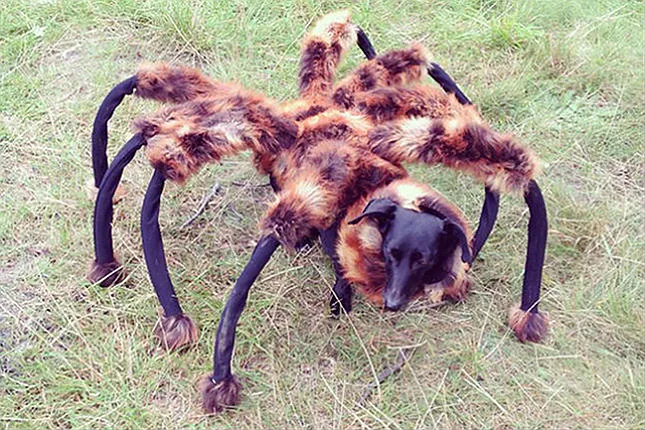
\includegraphics[width=1\textwidth]{Pictures/piespajak.jpg}
    \caption{Pies pająk standing still.}
    \label{fig:piespajak}
\end{figure}
\vspace{0.1cm}
\newpage
\section{Aleksander Trzciński}

The well known Pythagorean theorem:
\\
\(a^2 + b^2 = c^2\) 
\\
In physics, the mass-energy equivalence is stated 
by the equation:
\\
\(E=mc^2\).
\\
From the above equations it follows that:
\\
\(E=m(a^2 + b^2)\)

Photo~\ref{fig:IT meme}.
\begin{figure}[htbp]
    \centering
    
\includegraphics[width=1\textwidth]{Pictures/IT meme.jpg}
    \caption{Funny meme.}
    \label{fig:IT meme}
\end{figure}

\newpage

Table~\ref{tab:tabelunia}.
\begin{table}[htbp]
\centering
\begin{tabular}{|l|l|l|l|}
\hline
2 & 1 & 3 & 7 \\ \hline
6 & 7 & 6 & 9 \\ \hline
0 & 4 & 2 & 0 \\ \hline
6 & 6 & 6 & 6 \\ \hline
\end{tabular}
\label{tab:tabelunia}
\caption{matrix with random numbers}
\end{table}
\\
To buy list
\begin{itemize}
  \item tomatoes
  \item potatoes
  \item apples
\end{itemize}
\\
Numbered list:
\begin{enumerate}
  \item tomatoes
  \item potatoes
  \item apples
\end{enumerate}

\section*{Lorem ipsum}

\begin{flushleft}
\textbf{Lorem ipsum} \underline{dolor sit amet,} \textbf{\textit{consectetur adipiscing elit.}} Etiam lobortis vulputate ipsum sed tempus. Integer tincidunt ligula ipsum. Praesent volutpat eget justo nec euismod. Suspendisse potenti. Pellentesque quis molestie risus. Praesent nec ipsum et libero pharetra tempus quis sit amet odio. Nulla ultrices sem pellentesque tincidunt hendrerit. Nam venenatis sit amet urna at viverra. Aenean ut sagittis orci.\par Class aptent taciti sociosqu ad litora torquent per conubia nostra, per inceptos himenaeos. Nunc sollicitudin magna neque, vel tempus est facilisis sed. Quisque pretium pellentesque diam, quis tempus neque. Phasellus magna augue, malesuada ut cursus porta, efficitur ut turpis.
\end{flushleft}

\section*{Ut vestibulum lectus}

\begin{flushleft}

Ut vestibulum lectus sed ipsum sollicitudin, eu sagittis magna fermentum. Pellentesque bibendum leo sit amet orci vulputate porta. Duis non commodo ipsum. Morbi vitae pretium nibh. Ut viverra est id pretium ornare. Praesent at congue lorem, sed faucibus dui. Suspendisse vel mauris est. Vivamus vehicula interdum ligula et pharetra.\par Integer sed nisi euismod, ultrices ipsum ut, laoreet magna. Nulla elementum neque nunc, a ultricies sem porta non. Mauris scelerisque in eros et ullamcorper. Morbi auctor laoreet faucibus. Proin congue sem et enim eleifend lacinia. Nullam ac sollicitudin orci, quis finibus odio. Cras at lectus ut justo tincidunt lacinia.
\end{flushleft}


\vspace{0.1cm}
\input{Chapters/chapter5_Natalia_Kwiecień.tex}

Photo~\ref{fig:piespajak}.
\begin{figure}[htbp]
    \centering
    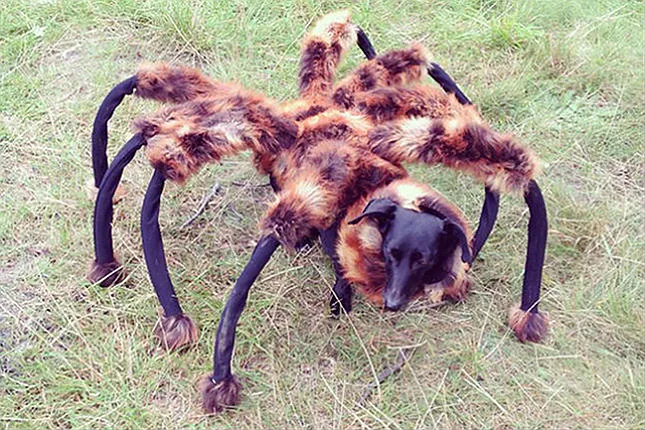
\includegraphics[width=1\textwidth]{Pictures/piespajak.jpg}
    \caption{Pies pająk standing still.}
    \label{fig:piespajak}
\end{figure}

\end{document}
